\documentclass[a4paper]{article}
 
\usepackage{amsmath}
\usepackage{graphicx}
\usepackage{caption}
\DeclareCaptionFont{white}{\color{white}}
\DeclareCaptionFormat{listing}{\colorbox{gray}{\parbox{\textwidth}{#1#2#3}}}
\captionsetup[lstlisting]{format=listing,labelfont=white,textfont=white}



\usepackage{subfigure}
\usepackage{epstopdf}
\usepackage[ansinew]{inputenc}
\usepackage{listings}
\usepackage{xcolor}
%\setlength{\oddsidemargin}{0cm}
%\setlength{\evensidemargin}{0cm}
%\setlength{\topmargin}{0cm}

\usepackage[]{algorithm2e}

\usepackage{a4wide}
\usepackage{pgfplots}
\pgfplotsset{compat=newest}

\title{ Simulating the mouse brain model constructed from Allen Institute for Brain Science data on the Blue Brain 4 supercomputer }
\author{Till Schumann}
%\date{}

\begin{document}
   \maketitle

\section{Introduction}
In 2014, the Neurorobotics team of the Blue Brain Project (BBP), project of the Ecole Federale Polytechnique Federale de Lausanne (EPFL), successfully produced a point-neuron model
of a mouse brain from data provided by the Allen Institute for Brain Science (Provide reference of Allen Institute).
Using NEST software, the BBP Neurorobotics team was then able to simulate a
scaled-down model of the mouse brain on a laptop computer, paving the way towards
making a mouse brain interact with an environment. A full-scale implementation of
the mouse brain model is possible, but requires the of large scale resources with low latency requirements only modern supercomputers can today provide.
The current functionality of NEST supports  generating large neuronal networks
on a super computer based an random distributions but not yet from experimental data contained in brain atlases. 
We suggest as part of this thesis to first develop the means to fully model a mouse brain from experimental data using NEST software on available supercomputing architectures.
\newpage

\subsection{Brain Simulations}
\subsection{Anatomy of the brain}
 
 The human brain is the main part of the central nervous system
 which consists of the spinal cord, sensory organs
 and all of the nerves that connect these organs with the rest of the body.
 These organs are responsible for the control of the body and communication between its parts.
 The nervous system is the most complex system of our body with respect to functionality.
 It contains billions of nerve and glia cells. 
 The nerve cells are connected via synapses to a complex network.
 Electrical pulses from neuron to neuron transmit information through the network.
 Glia cells help to maintain the right concentration of chemical substances in the
 extracellular space around neurons and provide supporting structures for the
 growth of neurons and for their spatial arrangement.
  \subsubsection{Macroscopic structure}
  \label{sec:Macroscopicstructure}
  The anatomy of the brain as depicted in Figure \ref{Aufbau1}, shows that different parts vary in cell density and functionality.
 Figure \ref{Aufbau1} shows a cross-section of the human brain. The outer layer is called the gray matter, due to the color caused by the high density of nerve cells.
 The white matter, which is underneath the gray matter,
 consists most of connection fibers of the nerve cells.
 The thalamus is situated in the middle of the brain and functions as a relay station between the sensory system and the cortical systems for cognition and motor control.
  \begin{figure}[!htbp]
  \subfigure[A cross-section of the human brain shows different densities of nerve cells \cite{CN}.]{
  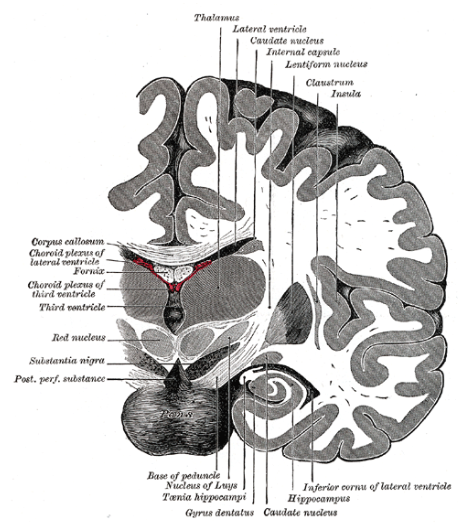
\includegraphics[scale=0.3]{Aufbau1.png}
  \label{Aufbau1}
  }
  \hfill
  \subfigure[A general map of the human brain assigns parts of the gray matter to fuctionalities \cite{CN}.]{
  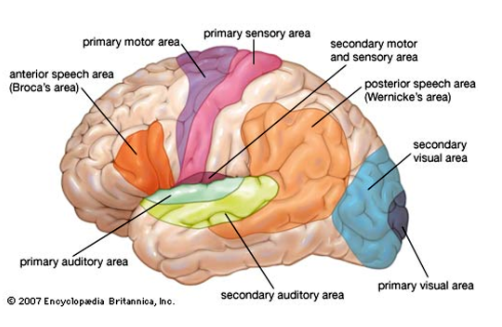
\includegraphics[scale=0.3]{Aufbau2.png}
  \label{Aufbau2}
  }
  \hfill
  \subfigure[The vertical structure of the gray matter shows six layers \cite{CN}.]{
  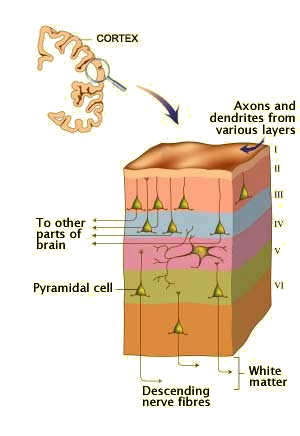
\includegraphics[scale=0.3]{mikro_aufbau.png}
  \label{mikroaufbau}
  }
  \caption{The macroscopic structure of the human brain.}
  \end{figure}
  Because of the high density of nerve cells the gray matter is the main part of information processing of the brain.
  
  The number of nerve cells (neurons), the number of connections (synapses) and the structure differs from person to person.
  The connections of each neuron are dynamic and change over time.
  Some parts of the brain can still be assigned roughly to functionality as shown in Figure \ref{Aufbau2}.\\
  Having a look at the vertical structure of the cortex,
  the gray matter can be partitioned in six layers as shown in figure \ref{mikroaufbau}.
  The cells in each layer have similarities like cell type, connections to other layers and connections to the thalamus and other parts.
  %-forebrain(anterior part of the brain)
  %-neocortex(surface of the mammalian brain, gray)
 
 
  \newpage
  \subsubsection{Microscopic structure}
  The nerve cells are tiny structures which are connected to each other.
  For an understanding of the brain a deeper look at the nerve cells is necessary.
  There are different cell types in a brain. They vary in structure and size.
  Pyramidal, spiny stellate and smooth stellate cells occur most often.
  For each layer there are types which occur more frequent. 
  
  In Figure \ref{Corticalneurons} a typical neuron is depicted.
  It contains the soma (the cell body) dendrites and axons.
  Electrical pulses are transported from the dendrites to the soma.
  In case of a spike an electrical impulse is forwarded through the axon.
  These axons are connected via synapses to further dendrites.
  The electrical impulse is transmitted via a chemical reaction in the synapse to the dendrites of connected cells.
  \begin{figure}[!htbp]
    \centering
    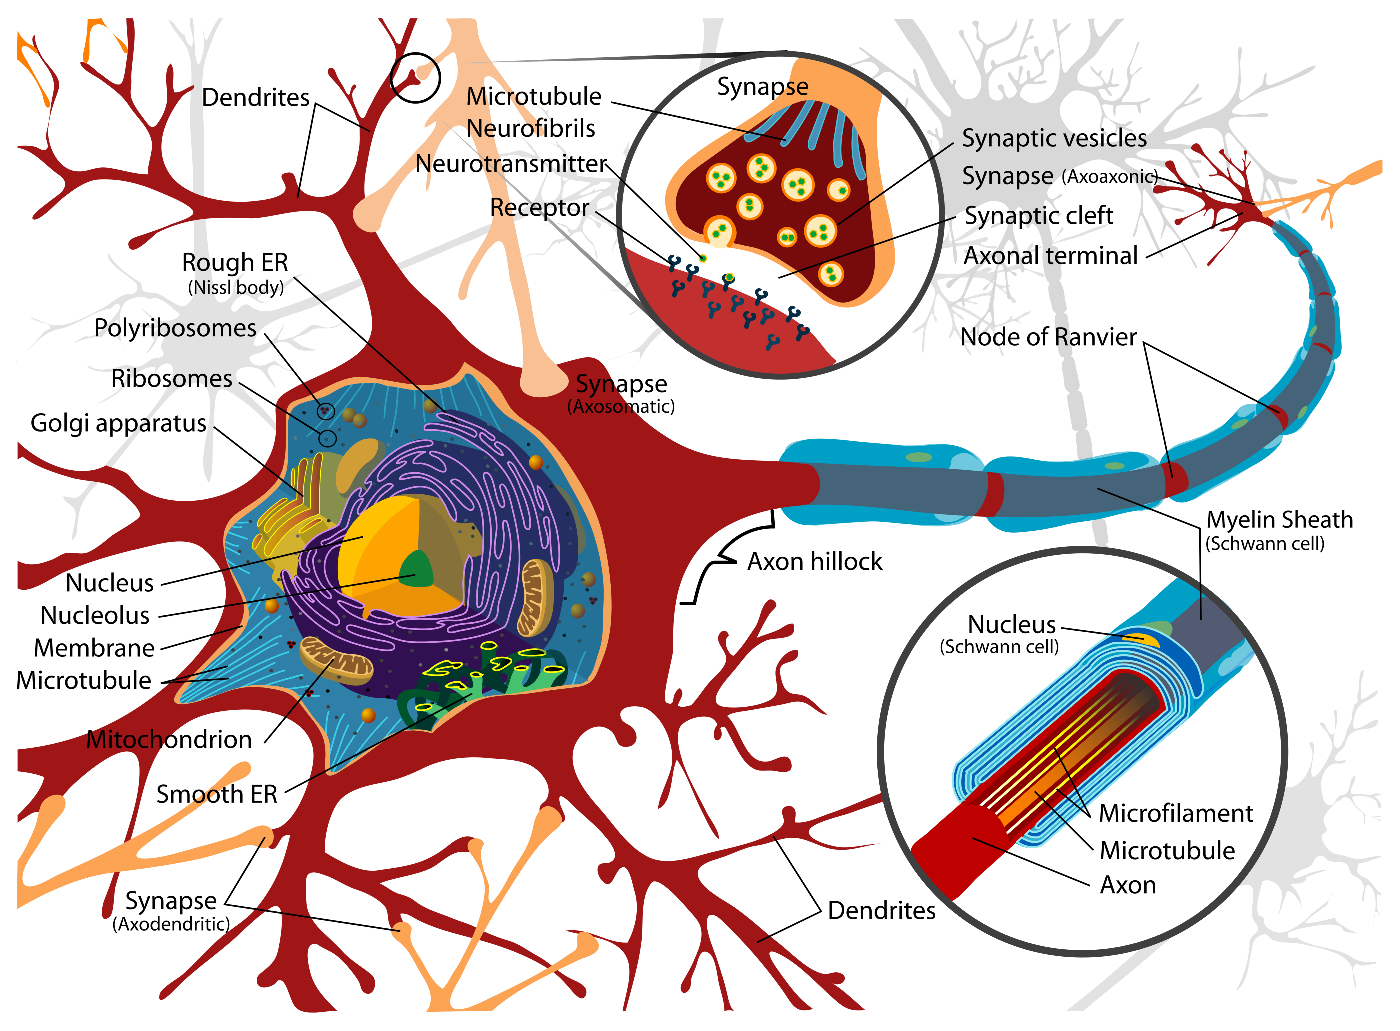
\includegraphics[scale=0.65]{Complete_neuron_cell_diagram_en.eps}
    \caption{Microscopic structure of a neuron. \cite{neuronpic}}
    \label{Corticalneurons}
  \end{figure}
  There are excitatory and inhibitory neurons.
  The excitatory neurons excite the following neurons, 
  in contrast the inhibitory neurons inhibit the following neurons.
  Via electrical currents the connected neurons influence the membrane potential of each neuron.
  The membrane potential can be measured.
  As an example the membrane potential is plotted over time in Figure \ref{membrane_potential}.
  Chemical processes inside the neuron generate a spike if the membrane potential reaches a specific electrical level called the threshold.  
  As shown in Figure \ref{membrane_potential} spikes are peaks in the membrane potential.  
  
  %-cortical neurons
  %-different cells: pyramidal, spiny stellate, smooth stellate
  %-cortical layers
  %-synapses
  
  %-10e12 neurons in the human brain
  \newpage
  \begin{figure}[!htbp]
  \subfigure[The plot shows the membrane potential of a neuron over the time.
  The peaks are called spikes.
  There are four spikes in the time span shown.
  The firing threshold of the cell is at about 58 mV \cite{CN}.]{
  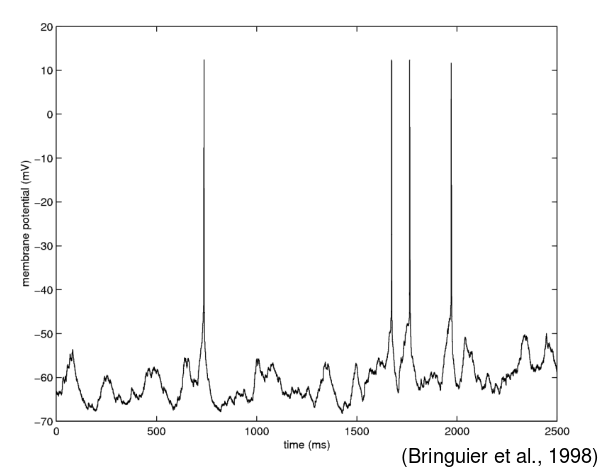
\includegraphics[scale=0.36]{membrane_potential.png}
  \label{membrane_potential}
  }
  \hfill
  \subfigure[The dot plot shows spikes of each neuron over time. On the y-axis there are the neurons number.
  The histogram in the lower panel sums up all spikes for each time bin. \cite{CN}]{
  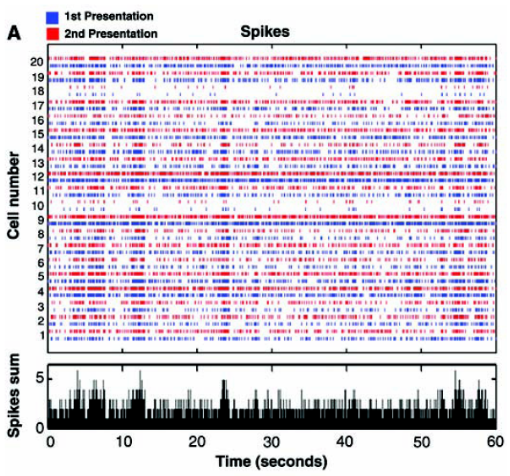
\includegraphics[scale=0.36]{spike_plot.png}
  \label{spikeplot}
  }
  \caption{The activity of a single neurons is displayed using its membrane potential. For multiple neurons the information is reduced to spike timings.}
  \end{figure}
  
  In order to analyze the membrane potential more objectively it is reduced to timings of the spikes.
  For multiple neuron the spike timings in a dot plot can be visualized as in Figure \ref{spikeplot}.
  One can get an overview of the activity in a whole neuronal network if the spike sums are
  plotted (summed up spikes for each time bin) in a so-called histogram.

	\begin{itemize}
      \item Short overview over simulators: NEST, NEURON, STEPS
      \item Possibilities/limits of simulations
   \end{itemize}
   
\subsection{Virtual mouse}
	\begin{itemize}
      \item Available data
      \item Why of interest
   	\end{itemize}   
\newpage
\subsection{Allen Brain Atlas}
   Allen Institute for Brain Science provides a high-resolution map of neural connections in the mouse brain.
   It contains several injection experiments. The provided datasets of the experiments 
   contain a 3D image of the injection and a 3D image of its axonal projection labeled by viral
   tracers.
   
   \begin{figure}[ht!]
   	\begin{center}
        \subfigure[Injection sites - showing all available experiments]{%
            \label{fig:allInjections}
            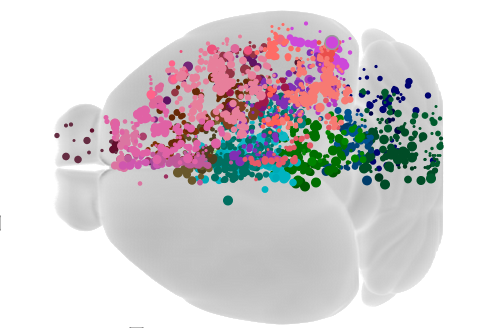
\includegraphics[width=0.4\textwidth]{../connectionBrowser_allinjections.png}
        }
        \hspace{1cm}
        \subfigure[Projection density of one experiment]{%
            \label{fig:oneProjection}
            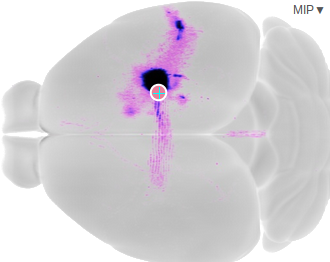
\includegraphics[width=0.32\textwidth]{../connectionBrowser_oneinjections.png}
       }
    	   \end{center}
    	\caption{%
        The pictures are inverted and copied from the Allen Brain Atlas.
     }%
   \label{fig:atlas}
   \end{figure}
   
   \begin{itemize}
      \item description
\end{itemize}
   
\subsection{BBP recipe}
\begin{figure}[ht!]
\centering
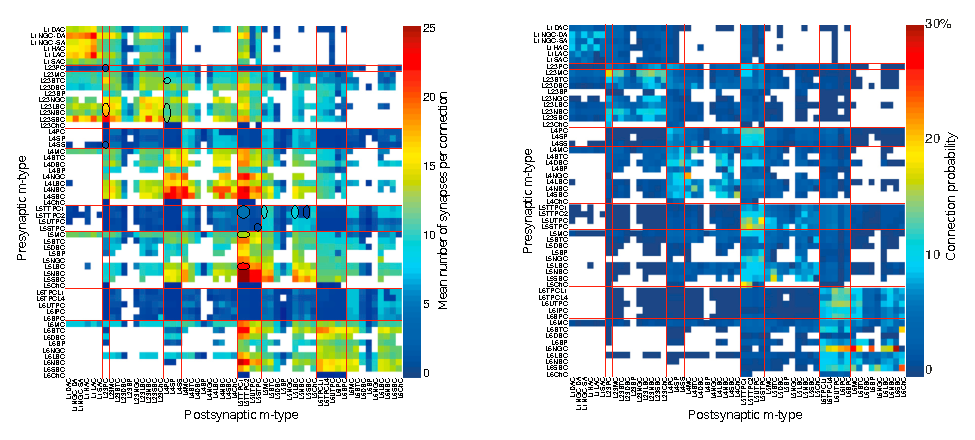
\includegraphics[scale=0.9]{BBPconnectionPropasMatrix.eps}
\end{figure}

\begin{itemize}
      \item description
\end{itemize}

\subsection{NEST}
NEST is a simulator for spiking neural network models that focuses on the dynamics, size and structure of neural systems rather than on the exact morphology of individual neurons. The development of NEST is coordinated by the NEST Initiative. NEST is ideal for networks of spiking neurons of any size, for example:
Models of information processing e.g. in the visual or auditory cortex of mammals, models of network activity dynamics, e.g. laminar cortical networks or balanced random networks and models of learning and plasticity. A NEST simulation tries to follow the logic of an electrophysiological experiment that takes place inside a computer with the difference, that the neural system to be investigated must be defined by the experimenter. The definition is based on number of neurons with parameters and connections between these neurons. NEST supports the generation based on probabilistic values. The stochastic settings of a neuronal network can be used to create its artificial copy inside of NEST. To manipulate or observe the network dynamics, the experimenter can define so-called devices which represent the various instruments (for measuring and stimulation) found in an experiment. These devices write their data either to memory or to file. 

\subsection{Visualization}
To interpret the output of a neuronal simulation the spiking activity of the neurons is analyzed, mostly. Different types of methods allow to extract stochastic characteristics from spike trains. Besides this visualization of the spike trains taking their location into account, allows to create a video, which shows the activity of the neuronal network.




\section{Analysis}

\subsection{Available resources}   
The Blue Brain 4 system is a set of tightly integrated high-performance resources. It is comprised of a four-rack IBM BlueGene/Q system 65 536 PowerPC A2 1.6 GHz cores for computing, providing a peak performance of 839 TFlops 65 TB of RAM, a shared parallel filesystem based on GPFS / GSS of a capacity in excess of 4 petabytes and a bandwidth exceeding 40GB/s A FDR Infiniband network Job scheduling across the system's components is performed by Slurm. 

\begin{itemize}
      \item Juelich
\end{itemize}


\subsection{NEST simulations}
The standard use-case for the NEST simulator is a stochastic-driven simulation. This means
that the circuit is characterized by stochastic parameters (e.g. number of synapses between neurons).
The circuit is build-up inside of NEST using only these parameters.
This means that the amount of need data is small. It allows to build-up large scale simulation
with a few arguments.

\begin{itemize}
      \item What is simulated
      \item Which is the result of a simulation
      \item Which resources are necessary and limiting factor memory
\end{itemize}

\subsubsection{Memory consumption of NEST}
The memory usage of the newest NEST release 2.6.0 can be calculated with following equation. \cite{kunkel2014spiking}
\begin{equation}
  \Pi(M,T,N,K) =  \Pi_0 + \Pi_n(M,N)  + \Pi_c(M,T,N,K)
  \label{eq:NESTmemconsumption}
\end{equation} 
\begin{equation}
  \Pi_n(M,N) = N_M*1100
\end{equation}
\begin{equation}
  \Pi_c(M,T,N,K) = 0.33 * T * N + T * N^1_c * 24 + T*(N-N^1_c)*128 + N_M*K*52
\end{equation}
$\Pi$ is the memory consumption. $\Pi_0$ is the initial memory consumption of NEST.
For the \emph{JUQUEEN} its around 26 MB and for \emph{K} around 260 MB.
$M$,$T$, $N$, $K$ correspond to number of MPI Nodes, number of threads per node, number of neurons and number of outgoing connection per neuron.
For the calculation there are some simplifications done.
The model uses the \emph{iaf\_psc\_alpha} neuron model for all neurons. There are only static synapses.
The number of incoming connection per neuron $K$ is not known. Only the number of outgoing connections is known.
To get some results anyway, it is expected that they are similar.
Furthermore the term of expected number of neurons without any VP-local target is set to zero, which is the worst case for the consumption of memory.

\subsection{Interfaces}
\begin{itemize}
      \item How to set up a simulation
\end{itemize}

\subsection{Data-driven simulation}
As we generated the circuit in a preprocessing step. Neuron and point to point synapse information are given.
Thus we call it a data-driven simulation. We do not use the build-up functionality from NEST.
Hence we have to load the whole circuit from file.

\begin{itemize}
      \item parameters for each neuron
      \item in point to point connection information with parameters
   \end{itemize}

\newpage
\subsection{Circuit generation}
\begin{itemize}
      \item Create point circuit from available data
      \item Fuse data from the Allen Brain Atlas and the BBP recipe
   \end{itemize}

\subsubsection{Long range connections}
A set of experiments is used to connect neurons located at the injections
to the neurons at the projections. Unfortunately all injections from these experiments do not
cover the whole brain. So there are neurons which are not injected
by any experiment. Therefore all neurons which are not injected should use the projection
from the nearest injection. To map pixels of the 3D pictures to neurons, the neurons are assigned to voxels, which represent the pixels. In a first step the best experiment is chosen for each voxel based on the minimal total injection per experiment. In the second step all voxels in the right hemisphere, which have not received an experiment take the experiment from the nearest voxel, which has an experiment. In the third step the given experiments are used to generate the connections for the related neurons. To get connection for the both hemispheres the information is mirrored along the z-axis.

\begin{figure}[ht!]
   	\begin{center}
        \subfigure[Illustration injection]{%
            \label{fig:allInjections}
            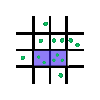
\includegraphics[width=0.15\textwidth]{cg_illustration_injection.eps}
        }
        \hspace{0.5cm}
        \subfigure[Illustration projection]{%
            \label{fig:oneProjection}
            
\includegraphics[width=0.15\textwidth]{cg_illustration_projection.eps}
       }
       \hspace{0.5cm}
       \subfigure[Merge experiment]{%
            \label{fig:allInjections}
            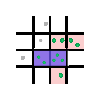
\includegraphics[width=0.15\textwidth]{cg_illustration_merge.eps}
        }
        \hspace{0.5cm}
        \subfigure[specify source and target neurons]{%
            \label{fig:oneProjection}
            
\includegraphics[width=0.15\textwidth]{cg_illustration_neurons.eps}
       }
    \end{center}
    	\caption{%
        Assign density of experiments to neurons.
     }%
   \label{fig:atlas}
   \end{figure}
   
   \begin{algorithm}
	\KwData{Injection experiments}
	\KwResult{Long range synapses}
	\For{each neuron n , identify the corresponding rAAV injection experiments}{
		Keep the experiment with the lowest injection volume; \\
		Select all neurons in the projection area; \\
		Assign each of them the normalized intensity value $D_i$ of the voxel they are situated in \\
		Generate a random number P between 0 and 1; \\
		Pick randomly a neuron i; \\
		\If{$P < D_i$}{
			Create an efferent synapse from the selected neuron to neuron $i$; \\
			Assign synaptic parameters; \\
		}
		Repeat from step 4) until Nsy=10000 efferent synapses are created;
	}
\label{alg2}
\caption{Generate long range connectivity}
\end{algorithm}
   
   \begin{itemize}
      \item Implementation
      \item Parallel efficiency, memory consumption and limits
   \end{itemize}
   
\subsubsection{Short range connections}
The Blue Brain Project has investigated over the last years in experiential work the relation of different synapse types.
They collected their findings in a recipe which allows to get the synapse type for different neuron types.
The neuron types depend on their layer, electrical and morphological type. The recipe defines which synapses are between 
which kind of neurons. The generated synapses connect neurons to its neighborhood. The neighborhood is defined as a
column in the same orientation as the neuron has.


\begin{figure}[ht!]
   	\begin{center}
        \subfigure[contain all neuron information]{%
            \label{fig:shortColumn}
            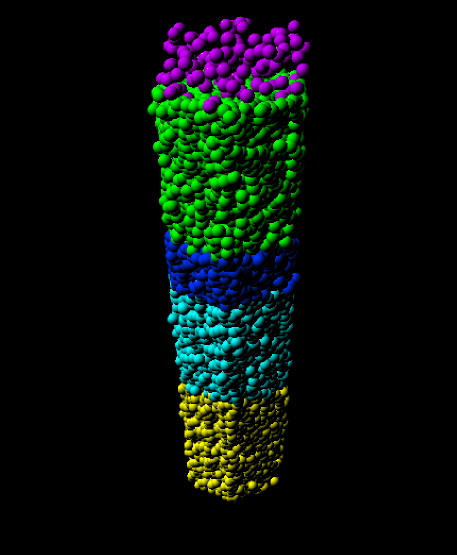
\includegraphics[width=0.22\textwidth]{../shortrange/g3111.png}
        }
        \hspace{0.5cm}
        \subfigure[contain all synapse information]{%
            \label{fig:shortColumnInCircuit}
            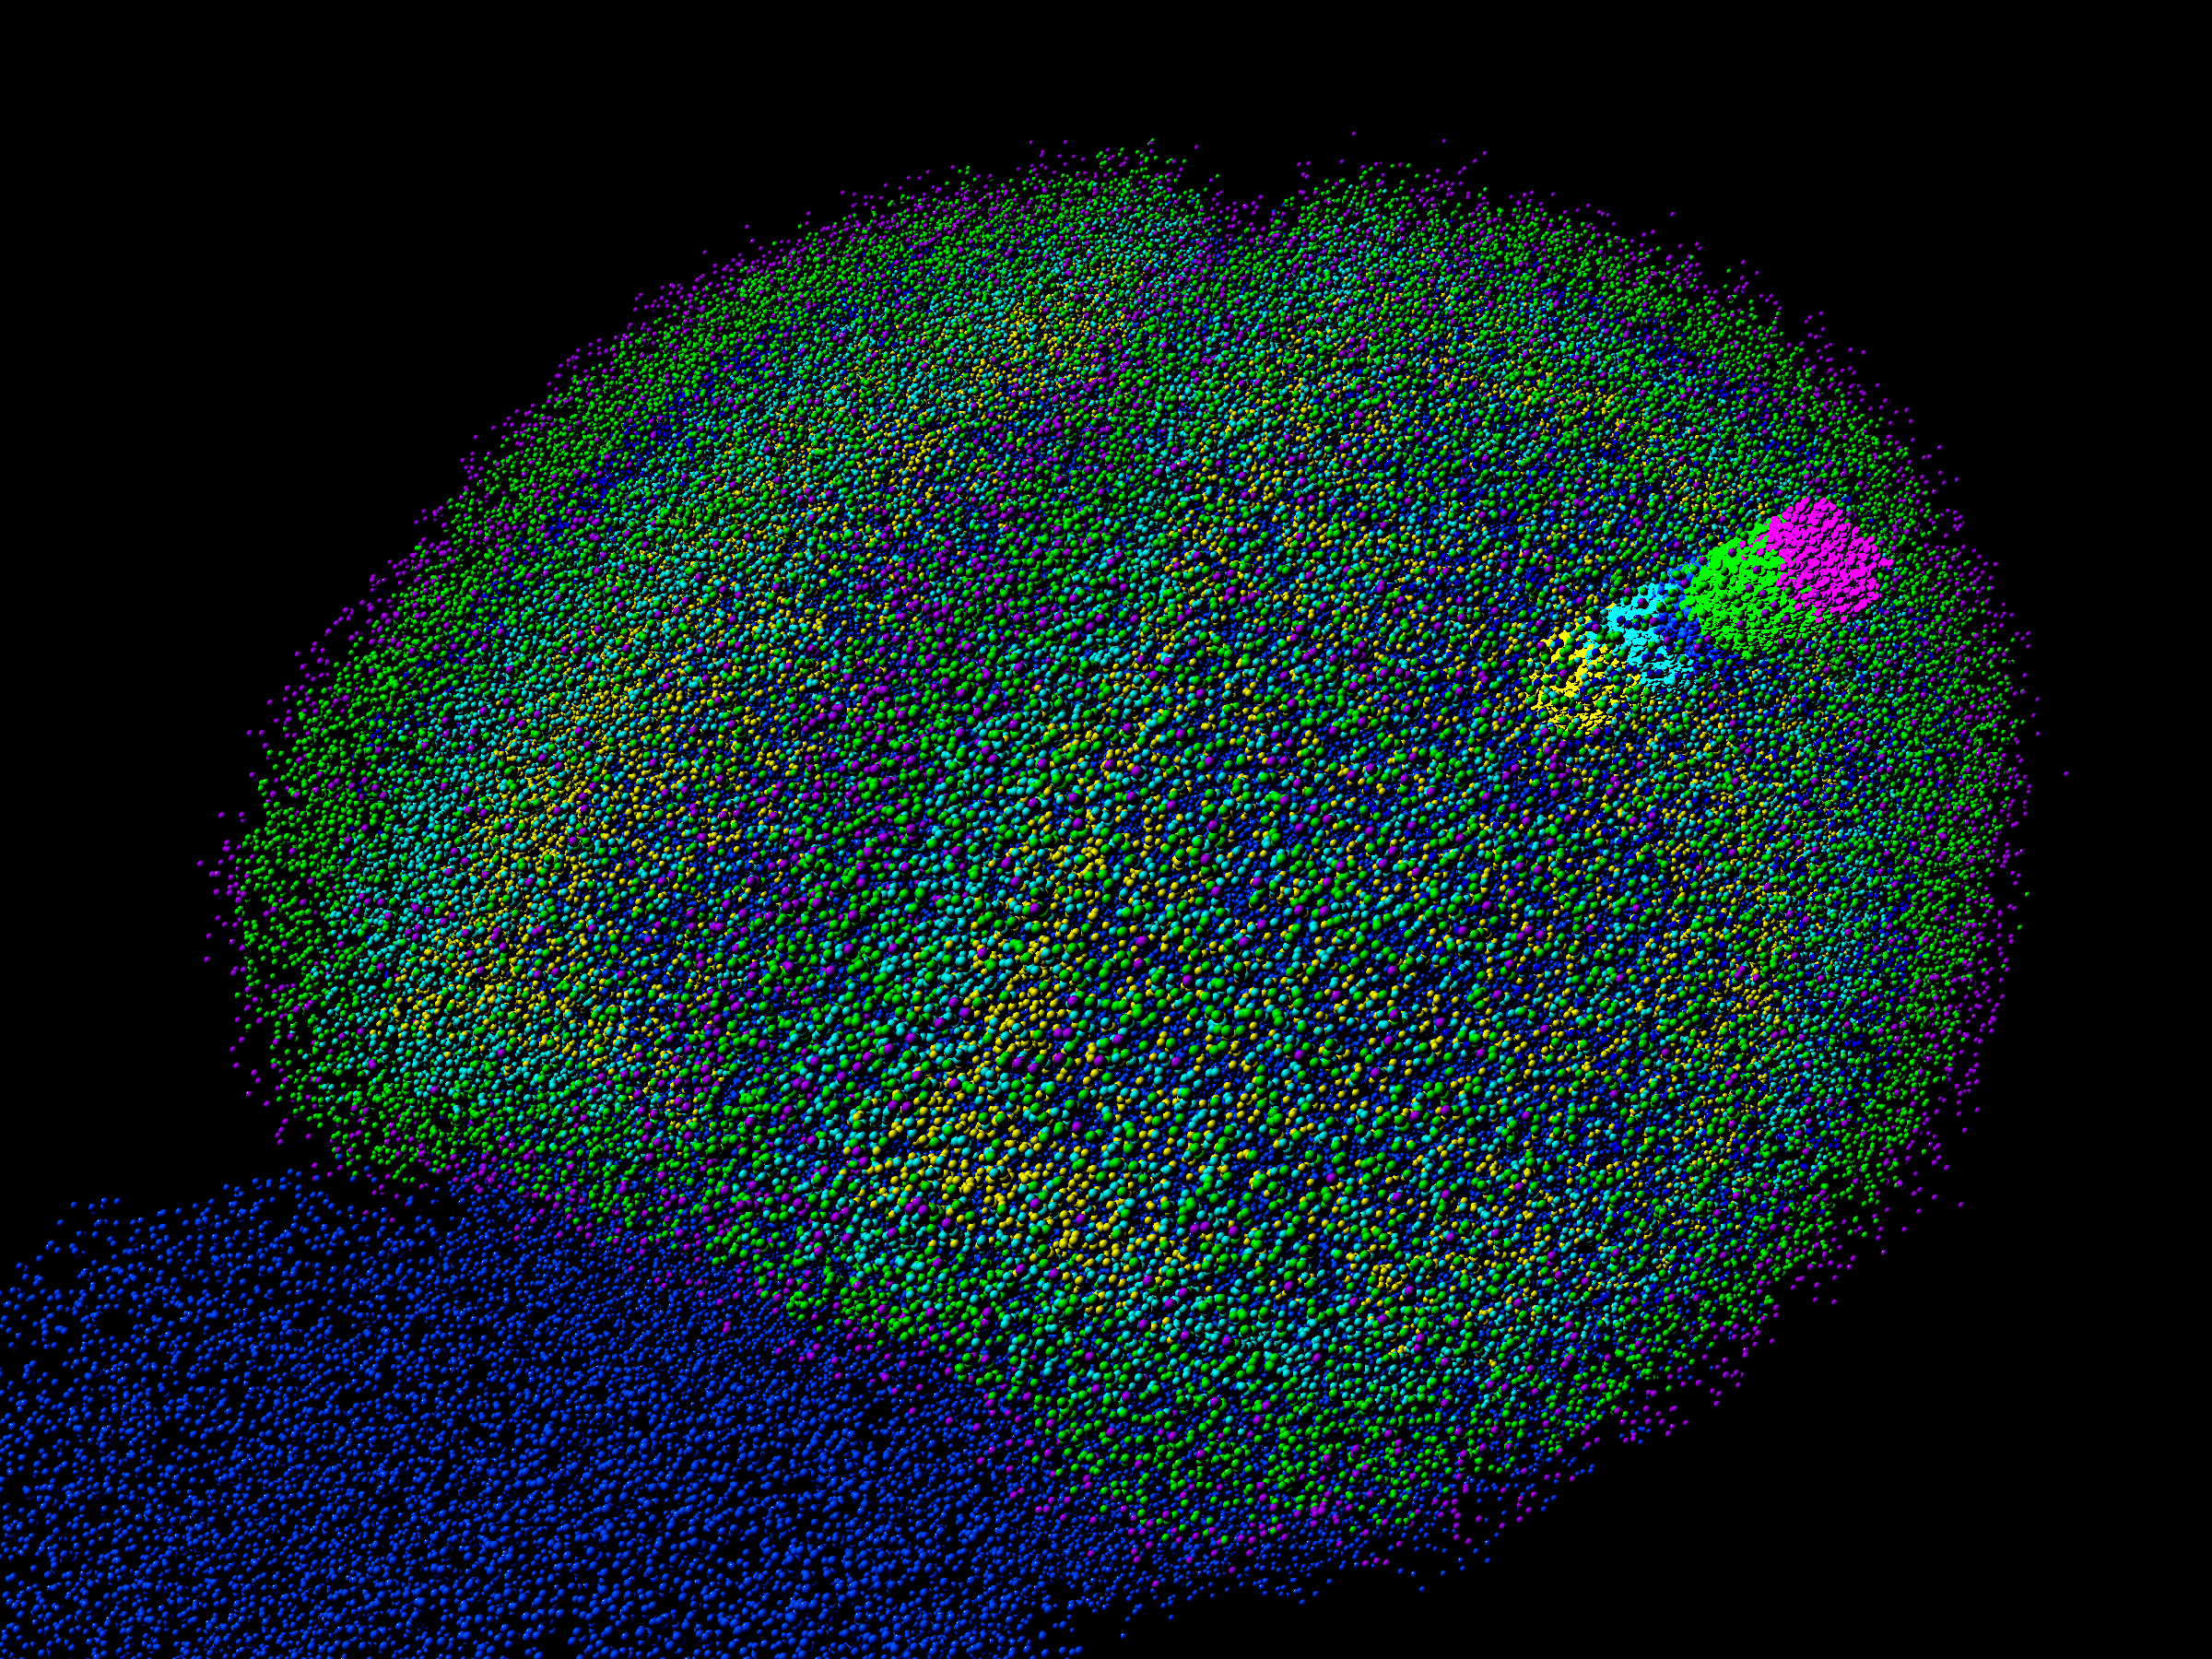
\includegraphics[width=0.34\textwidth]{../shortrange/column_in_brain_4_edit.png}
       }
        \hspace{0.5cm}
        \subfigure[illustration of neurons on grid]{%
            \label{fig:shortColumnInCircuit}
            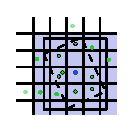
\includegraphics[scale=2.5]{illustration_shortrange_select.eps}
       }
  
    	   \end{center}
    	\caption{%
        3D visualization of the original Blue Brain Project column (left) and the reconstructed mouse
isocortical column that has a similar neuron density (right). Layers 1, 2/3, 4, 5 and 6 are
shown in different colors.
     }%
   \label{fig:atlas}
   \end{figure}
   
   \begin{algorithm}
	\KwData{BBP matrices}
	\KwResult{Short range synapses}
	\For{each neuron n}{
		Select all neurons in neuron $i$ column area; \\
		Generate a random number P between 0 and 1; \\
		Pick randomly a neuron j from selected area; \\
		Determine $D_i$ based on BBP matrices (neuron i properties, neuron j properties); \\
		\If{$P < D_i$}{
			Create an efferent synapse from neuron $i$ to neuron $j$; \\
			Assign synaptic parameters; \\
		}
	}
	\label{algshort}
	
	
\caption{Generate short range connectivity}
\end{algorithm}

\begin{itemize}
      \item Implementation
      \item Parallel efficiency, memory consumption and limits
   \end{itemize}

\subsection{Parallel IO}
Build-up a large scale neuronal network from point to point connectivity results in new requirements for data processing and the data format. The parallel IO is strictly limited by the given bandwidth. Clumsy parallel IO access can even lower the resulting bandwidth.
Thus the distribution of the parallel loading has to be carefully chosen. HDF5 allows parallel access to one file.
It uses MPI-IO to manage parallel read and write operations. Further HDF5 is a self descriptive format and therefore easy to handle
and exchanged between different platforms. Already given reduced circuits are stored in HDF5 file format by the neurorobotics team, 
because of its easy to use Python interface. On a personal computer a light weight python implementation allows to load a given
circuit from HDF5 to NEST, using HDF5 Python interface with the NEST python interface. Therefore selecting the same or similar data 
format is preferred to reduce the number of needed adaptions of scripts.


\subsubsection{HDF5}

\begin{figure}[ht!]
   	\begin{center}
        \subfigure[Hyperslab selection of HDF5 in a single dataset]{%
            \label{fig:shortColumn}
            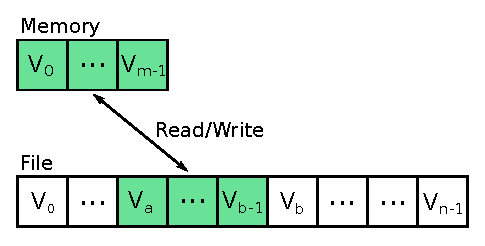
\includegraphics[scale=0.8]{HDF5Hyperslab.eps}
        }
        \hspace{0.5cm}
        \subfigure[Using hyperslab functionality to read or write dataset in parallel]{%
            \label{fig:shortColumnInCircuit}
            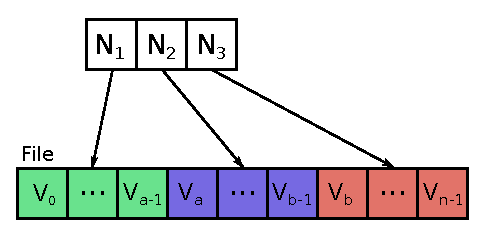
\includegraphics[scale=0.8]{HDF5Parallel.eps}
       }
  
    	   \end{center}
    	\caption{%
        Using HDF5 in parallel 
     }%
   \label{fig:atlas}
   \end{figure}


\subsection{Pipeline}
The requirements for all implementations are the usability for the scientists. Besides efficient implementation the users should be able to manipulate the data on different levels. Creating one simulation from data based on the Allen Brain Institute is not the main goal of this thesis. In fact the implementations should complete the tool chain to run data-driven simulations with NEST and visualize them, based on Allen injection experiments. Therefore the proposed pipeline contains data formats which can be manipulated. Processing the needed amount of data takes time and has to be executed on large compute clusters. Thus an interactive usage of the tools is not reasonable.

\newpage
\section{Implementation}

\subsection{Data format}

\begin{figure}[ht!]
   	\begin{center}
        \subfigure[contain all neuron information]{%
            \label{fig:allInjections}
            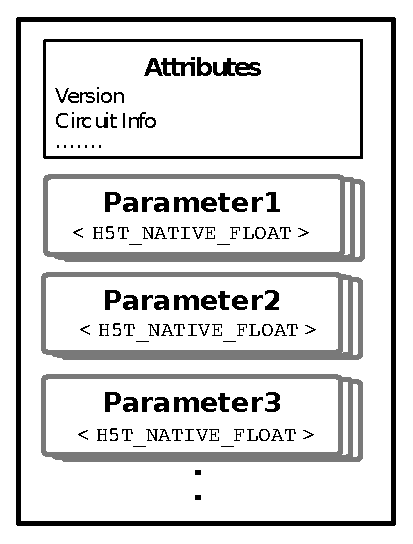
\includegraphics[scale=0.5]{hdf5_neuron_format.eps}
        }
        \hspace{1cm}
        \subfigure[contain all synapse information]{%
            \label{fig:oneProjection}
            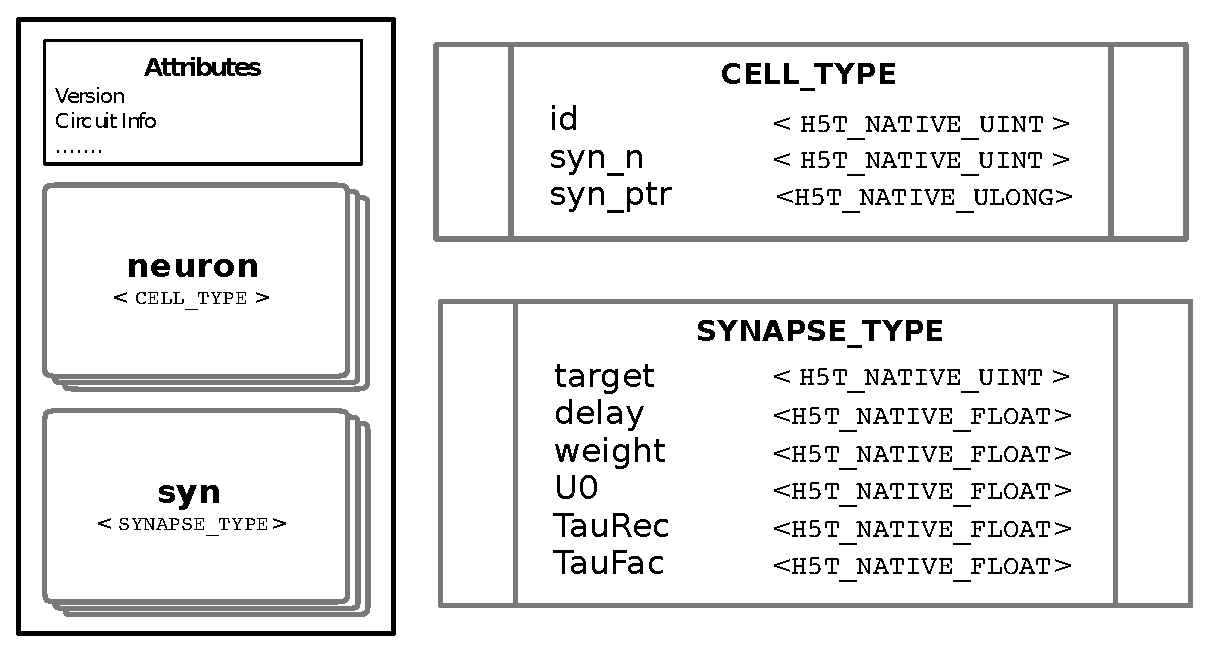
\includegraphics[scale=0.41]{hdf5_syn_format.eps}
       }
    	   \end{center}
    	\caption{%
        The HDF5 file formats.
     }%
   \label{fig:atlas}
   \end{figure}

\begin{itemize}
      \item Synapse data format
      \item Neuron data format
\end{itemize}

\subsection{Circuit generation}
Rewriting the sequential python script to a hybrid C++ application require a parallel implementation of a parallelization strategy and the usage of 
a parallel random generator. For the parallelization strategy a Master-Slave approach is chosen to distribute the workload dynamically on the nodes.
Communication between the individual nodes is not necessary. Only the workload management is handled by the master node.
For the random generator Random123 is used, because it has good performance and it is easy to use.
It ensures reproducible results without correlations in the generated values. 


\subsubsection{Long range connections}


\begin{itemize}
      \item parallelization strategy and implementation
      \item workflow diagram
      \item requirements 
\end{itemize}

\begin{figure}[ht!]
   	\begin{center}
        \subfigure[All nodes are equal and process the work based on a static distribution]{%
            \label{fig:shortColumn}
            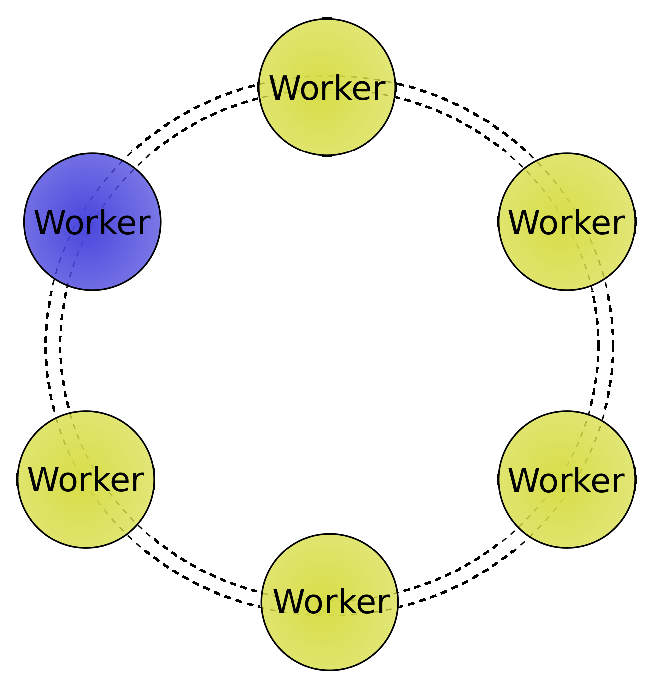
\includegraphics[scale=0.5]{All_Worker_Collective.eps}
        }
        \hspace{1cm}
        \subfigure[The 0 node is assigned as the master node and handles from this on the management of the work distribution.]{%
            \label{fig:shortColumnInCircuit}
            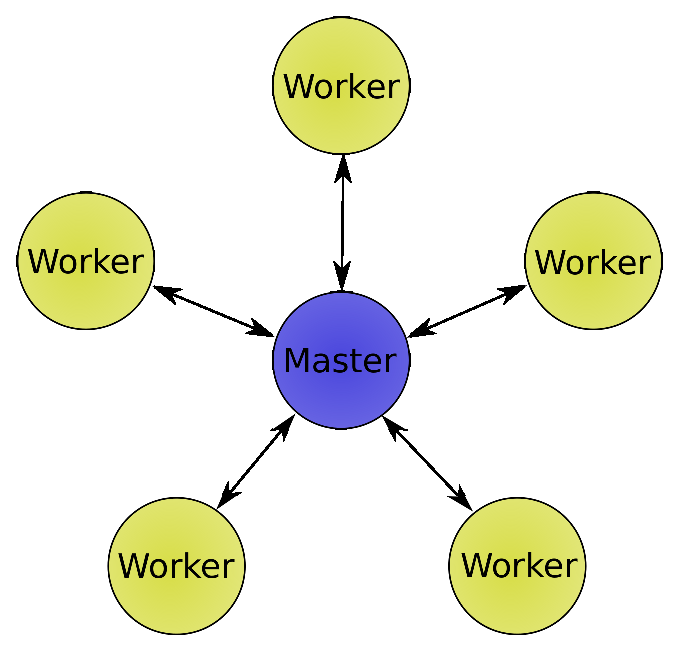
\includegraphics[scale=0.5]{MasterWorker.eps}
       }
    	   \end{center}
    	\caption{%
        The figure illustrates the work distribution and communication between the nodes.
     }%
   \label{fig:atlas}
   \end{figure}

\subsubsection{Short range connections}

The algorithm presented in the analysis section can be parallelized straight forward.
Each iteration is independent. The challenging part is the distribution of the iterations and
the writing to disk. The number ob synapses which are created is not know. It is only available
at the end.
\begin{itemize}
      \item parallelization strategy implementation
      \item workflow diagram
      \item requirements
\end{itemize}




\begin{figure}[ht!]
   	\begin{center}
        \subfigure[Master-worker strategy to get good balance properties]{%
            \label{fig:shortColumn}
            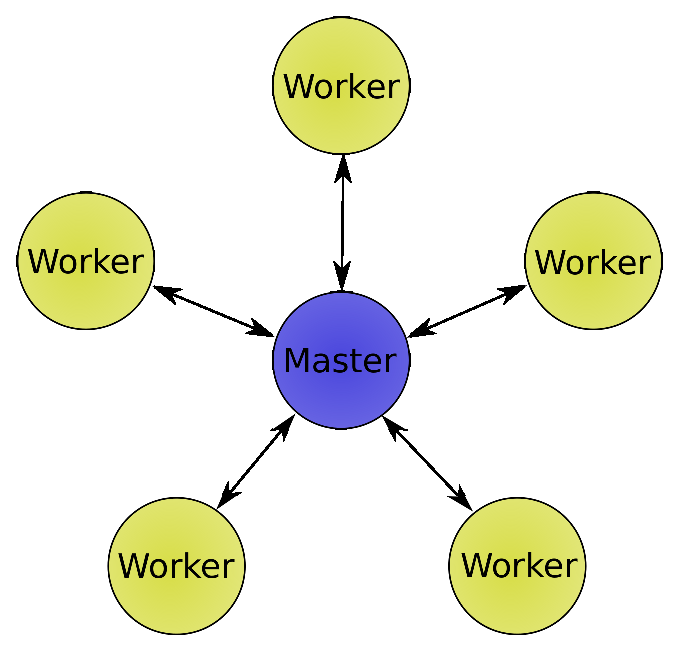
\includegraphics[scale=0.5]{MasterWorker.eps}
        }
        \hspace{1cm}
        \subfigure[Collective write operation to maximize used bandwidth]{%
            \label{fig:shortColumnInCircuit}
            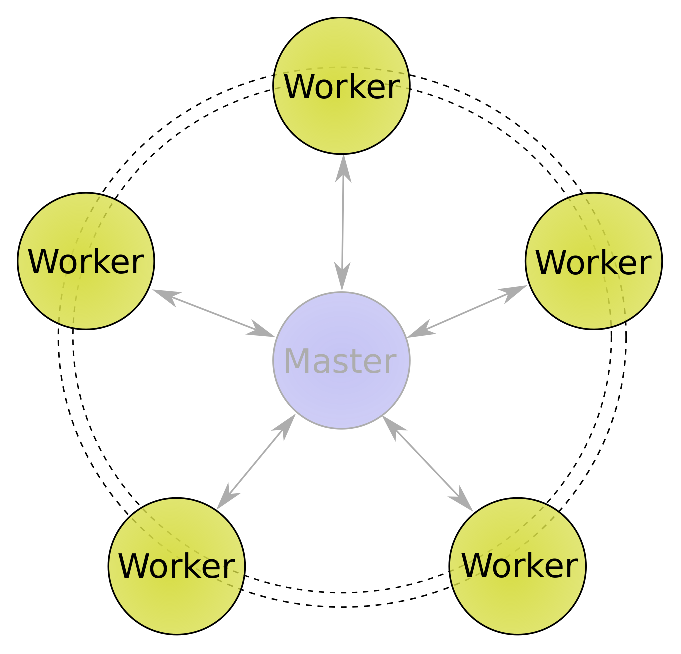
\includegraphics[scale=0.5]{Worker_Collective.eps}
       }
    	   \end{center}
    	\caption{%
        The figure illustrates the work distribution and communication between the nodes.
     }%
   \label{fig:atlas}
   \end{figure}


\subsection{Circuit validation}

In the context of this thesis the circuit is validated in terms of geometrical correct placement of
the synapses. So the position of the source and target can be visualized and be compared to a 
reference system. For the long and the short range connectivity the geometrical shape is know.
In particular the long range connectivity should connect neurons from the injected regions to neurons
in the projected region for every selected experiment. Therefore a circuit for a single experiment is 
generated, the target and source neurons are visualized in a 3D coordinate system and the the injection
and projection is used as the reference system. If source neurons are inside the injection space and all
target neurons are in the projection space, the implementation works fine.
For the short range connectivity all post-synaptic neurons of synapses having the same pre-synaptic neuron should
lay inside a cylinder in layer 1 to 6. For the validation. 
 
\begin{itemize}
      \item Visual validation of synapses to identify neuron id miss interpretation
      \item Visual validation of spiking activity
      \item Statistical properties are not analyzed in this work 
\end{itemize}

\begin{figure}[ht!]
\centering
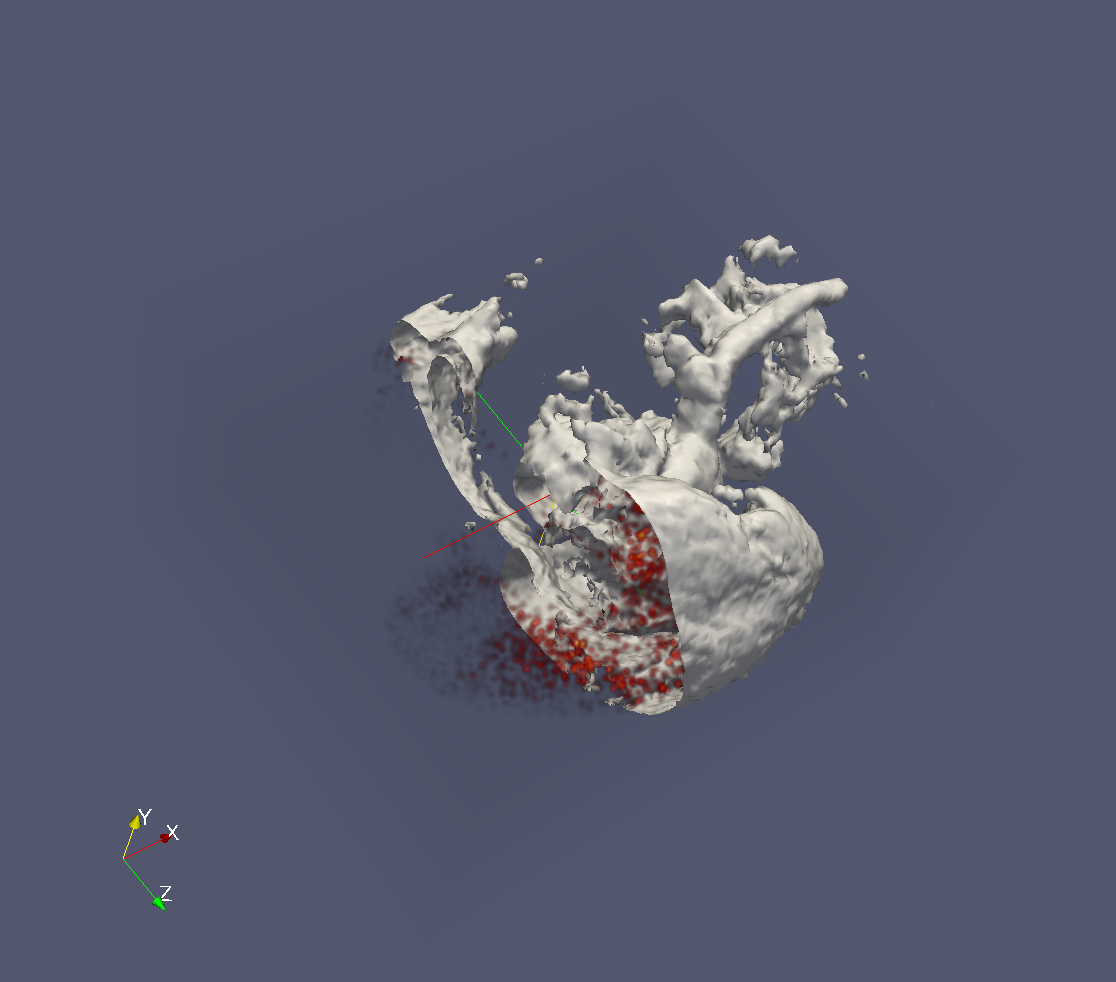
\includegraphics[width=0.4\textwidth]{paraview_ex.png}
\end{figure}

\subsection{NEST import module}

The neuronal spiking network simulator NEST is developed in \emph{C++} and delivers
an user interface based on an own description language \emph{SLI} and  and a Python interface.
The new use case shall be integrated into the standard work flow of NEST.
Besides the functionality in \emph{C++} the interfaces have to be extended.
The difficulties of the network generation is based on a difference in 
the NEST internal data structure and the data delivered by the Allen Institute.
Connection information contains target and source neurons besides biochemical
information of the synapses. Because of the in vitro injection methods the
connection information maps the synapse from the source to the target neurons.
For multi process simulations NEST distributes all neurons based on a modulo function 
to the processes. Because of memory optimizations the synapses are only stored on the
post synaptic process. This means that the connection information is stored
on the process, where the target neuron is located. Therefore a transformation of the given data is
necessary. Preprocessing of the input data should be avoided as far as possible to capture
future use cases.
The resulting implementation shall load the connection information efficiently in parallel,
distribute the synapse information to the post synaptic node and store it in
the NEST data structure.
Further requirements of the implementation are an efficient use of the available resources as
memory and computation power. 

\subsubsection{Algorithm}
The group data before send algorithm reads the the HDF5 file chunk wise.
Additionally the source neurons for each datasets (first row) are stored in a list.
So for all iterations the source neuron list is available in memory.
This source neuron list and the target neurons from each chunk are used to create a connection table.
It contains per connection one row with the source neuron in the first column and the target neuron in the second column.
The table will be sorted by the target nodes.
Using the \emph{MPI\_Alltoall} function this table can be distributed directly to the corresponding nodes.
Afterwards each node contains its connection table and calls the \emph{NEST} connection function.
\begin{algorithm}
	\KwData{List of HDF5 files for each node, chunk size}
	\KwResult{Connected NEST network}
	\While{Chunk to read in HDF5 files}{
		Read chunk and store in memory \hspace{45px}(1)\; 
		Create connection table [[$S_1$, $T_1$],[$S_2$, $T_2$],..] (1,2) \hspace{36px}$\mathcal{O}(n)$\; 
		Map target neurons to nodes \hspace{63px}(2,3) \hspace{36px}$\mathcal{O}(n)$\;
		Sort table by target neurons \hspace{66px}(2,3,*) \hspace{28px}$\mathcal{O}(n^2)$\;
		MPI\_Alltoall sorted data \hspace{76px}(2,3,4,5)\;
		Connect own connections in NEST \hspace{36px}(5) \hspace{45px}$\mathcal{O}(n)$\;
	}
\label{alg2}
\caption{Distribute connection information without transposing, $S_i$ source neuron $i$, $Tn_i$ target neuron $i$.
	set in brackets contains current needed variables}
\end{algorithm}

\begin{figure}[ht!]
\centering
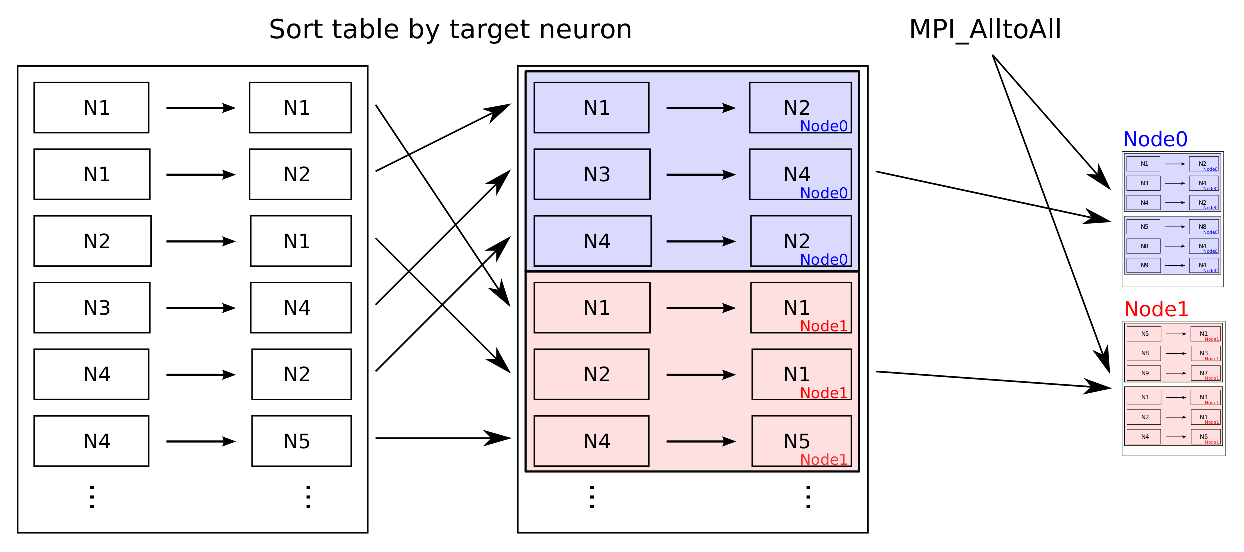
\includegraphics[scale=0.7]{sort_table_all_alltoall.eps}
\caption{Distribute synapses to the nodes.}
\end{figure}

\subsection{Memory consumption}
\begin{figure}[ht!]
\begin{tabular}{| l | l | l | l |}
    \hline
    (id) & data structures & memory consumption \\ \hline
    (1) & chunk in memory & $L_0 + h*(L_0 + L_S*w)$ \\ \hline
    (2) & connection table & $2*(L_0+L_S*w*s)$ \\ \hline
    (3) & target neuron node map & $L_0+L_S*w*s$ \\ \hline
    (4) & MPI send vectors & $L_0+L_S*2*w*s+2*(L_0+L_S*N)$ \\ \hline
    (5) & MPI recv vectors & $L_0+L_S*2*\frac{w*s}{\nu}+2*(L_0+L_S*N)$ \\ \hline
    \end{tabular}
\caption{$L_0$: constant memory overhead of list; $L_S$: memory consumption of entry type; $N$: number of nodes $w$: 1 dim of chunk; $h$: 2 dim of chunk; $DNC(w)$: replication of target neurons in chunk; $\nu$: distribution coefficient of data}
\end{figure}
The maximum memory consumption is:
\begin{equation}
  M = 9*L_0 + 4*L_S*N+L_S*w*s*(4+\frac{1}{\nu})
  \label{eq:maxmemoryconsumption}
\end{equation}

\newpage
\section{Discussion}
\subsection{Circuit properties}

\begin{figure}[ht!]
\centering
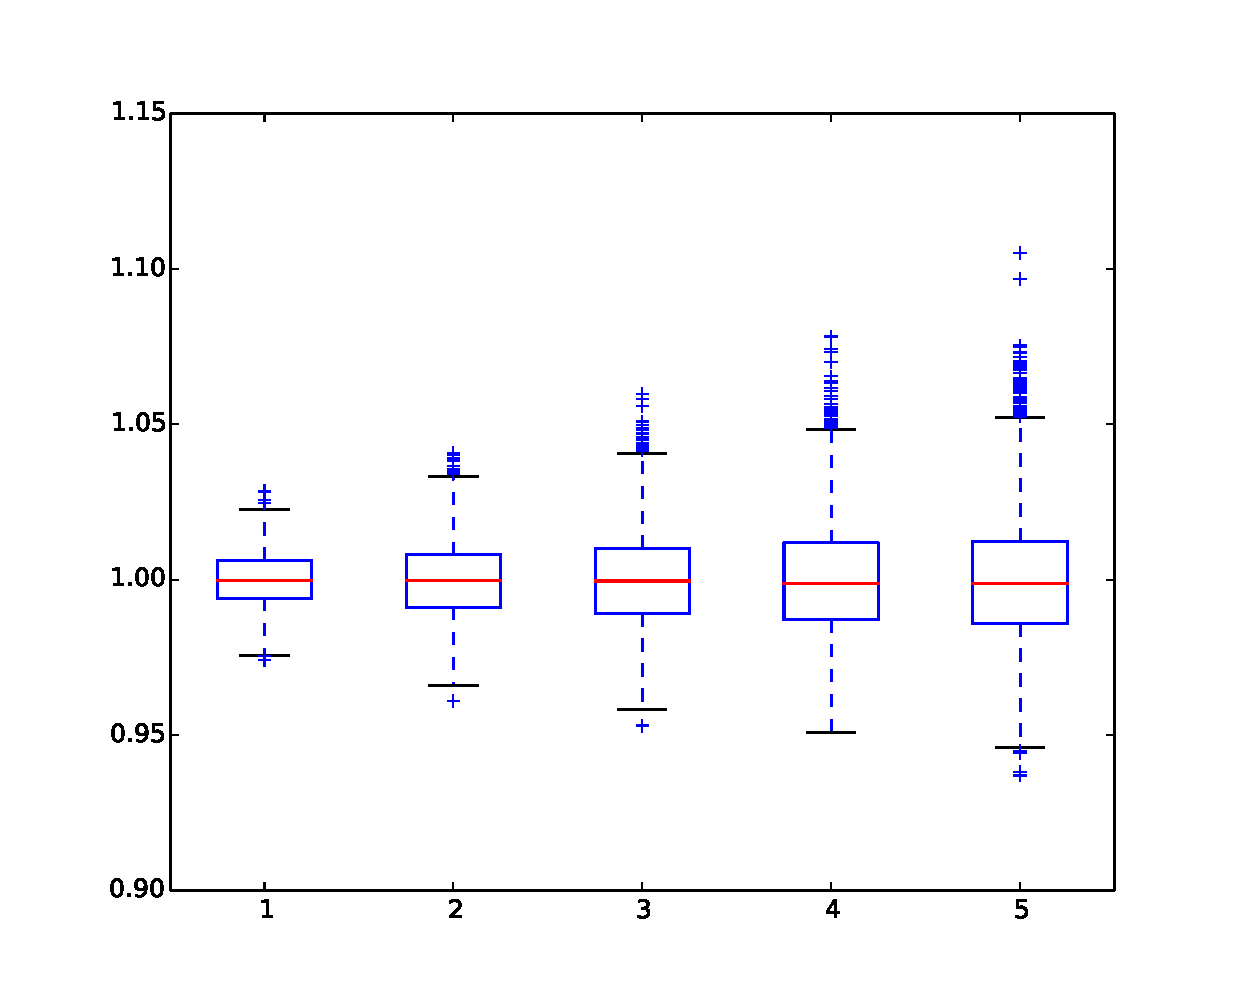
\includegraphics[scale=0.4]{full_circuit_rack_distribution.eps}
\caption{Synapse inbalance for using NEST standard configuration on different number ob nodes. The values are normalized by its mean value.}
\end{figure}

Memory imbalance resulting from an imbalance of number of synapses per neuron can be compressed by shuffling neurons on the nodes.
NEST distributes neurons based of the modulo of their ids. This results in a nearly equal number of neurons per node.
But it does not take the number of synapses per neuron into account. The distribution of ids can not be affected, but the assignment of the
neuron ids can be adjusted. Such a assignment implicate a memory overhead. The mapping has to be stored in memory and to disk for post processing.
If the memory overhead is bigger than the memory imbalance, there is no meaning in its implementation.

\begin{itemize}
      \item Scale of mouse brain
      \item Based on measured settings
      \item Contains interpolation data
      \item Easily adaptable, when more information are available
\end{itemize}

The 


\subsection{Data format usability}

The HDF5 data format for neuron parameters is used as given from the Neurorobotics team.
Because of its small size (9 GB) in comparison to the synapse dataset (15 TB) the performance improvement by changing
to a transposed data format can be neglected. Thus the usability of having different datasets and being able
to add new datasets can be kept. It also implies that the generation script does not have to be converted or no 
conversion scripts are needed.

\begin{itemize}
	  \item Neuron data format - performance vs usability
      \item Synapse data format - performance vs usability
\end{itemize}

\subsection{Parallel Efficiency}

\begin{figure}[!h] \centering
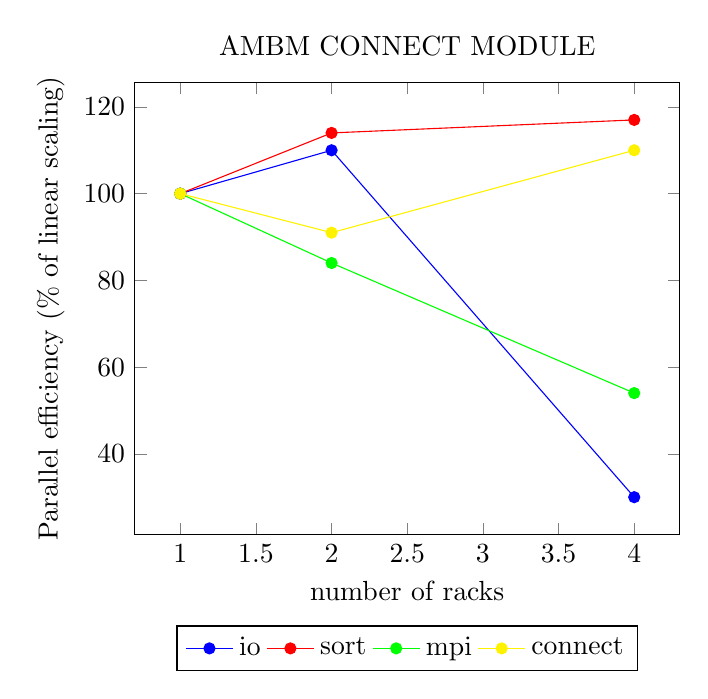
\begin{tikzpicture}
	\begin{axis}[title=AMBM CONNECT MODULE,
		legend style={at={(0.5,-0.20)},
		anchor=north,legend columns=-1},
		xlabel=number of racks,
		ylabel=Parallel efficiency (\% of linear scaling),
		width=8.5cm
		]

	\addplot[color=blue,mark=*] coordinates {
		(1,100)
		(2,110)
		(4,30)
	};
	\addplot[color=red,mark=*] coordinates {
		(1,100)
		(2,114)
		(4,117)
	};
	\addplot[color=green,mark=*] coordinates {
		(1,100)
		(2,84)
		(4,54)
	};
	\addplot[color=yellow,mark=*] coordinates {
		(1,100)
		(2,91)
		(4,110)
	};
	\legend{io,sort,mpi,connect}
	\end{axis}%
\end{tikzpicture}%
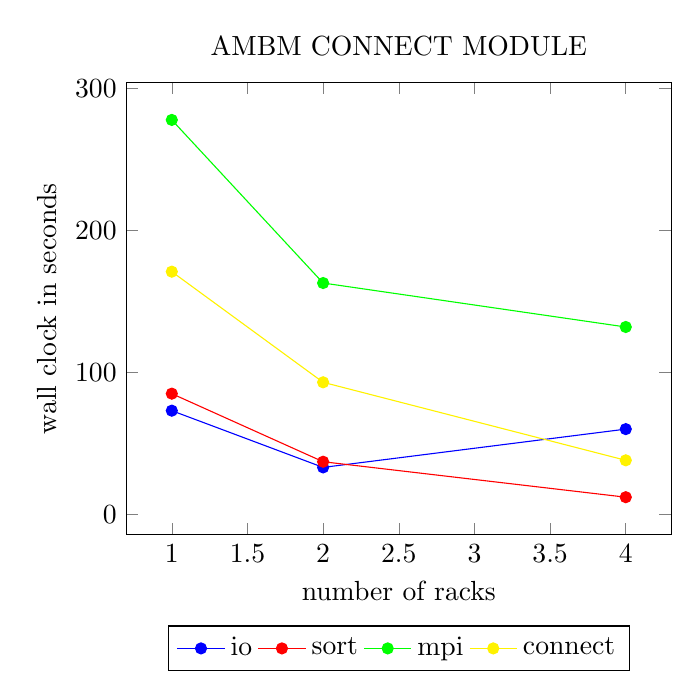
\begin{tikzpicture}
	\begin{axis}[title=AMBM CONNECT MODULE,
		legend style={at={(0.5,-0.20)},
		anchor=north,legend columns=-1},
		xlabel=number of racks,
		ylabel=wall clock in seconds,
		width=8.5cm
		]

	\addplot[color=blue,mark=*] coordinates {
		(1,73)
		(2,33)
		(4,60)
	};
	\addplot[color=red,mark=*] coordinates {
		(1,85)
		(2,37)
		(4,12)
	};
	\addplot[color=green,mark=*] coordinates {
		(1,278)
		(2,163)
		(4,132)
	};
	\addplot[color=yellow,mark=*] coordinates {
		(1,171)
		(2,93)
		(4,38)
	};
	\legend{io,sort,mpi,connect}
	\end{axis}%
\end{tikzpicture}%
\end{figure}
\begin{figure}[!h] \centering
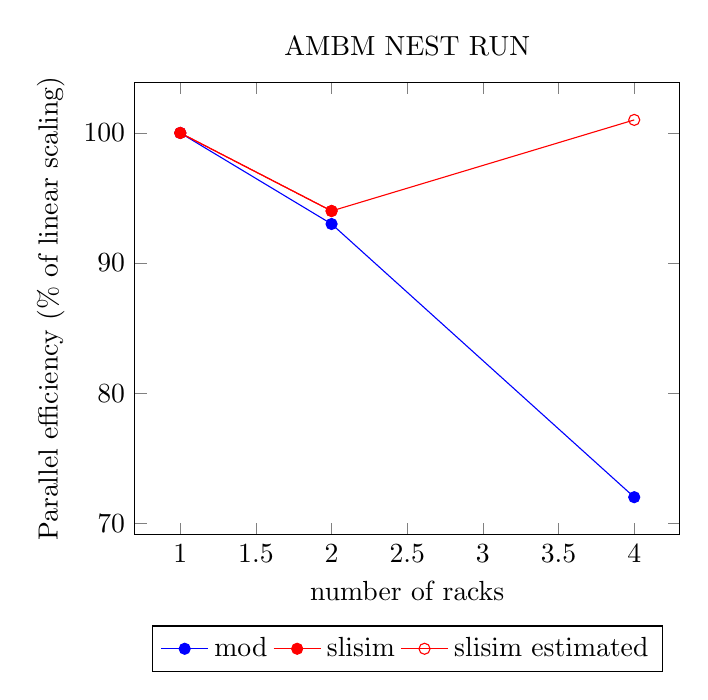
\begin{tikzpicture}
	\begin{axis}[title=AMBM NEST RUN,legend style={at={(0.5,-0.20)}, anchor=north,legend columns=-1},
		xlabel=number of racks,ylabel=Parallel efficiency (\% of linear scaling),width=8.5cm]

	\addplot[color=blue,mark=*] coordinates {
		(1,100)
		(2,93)
		(4,72)
	};
	\addplot[color=red,mark=*] coordinates {
		(1,100)
		(2,94)
	};
	\addplot[color=red,mark=o] coordinates {
		(1,100)
		(2,94)
		(4,101)
	};
	\legend{mod,slisim, slisim estimated}
	\end{axis}%
\end{tikzpicture}%
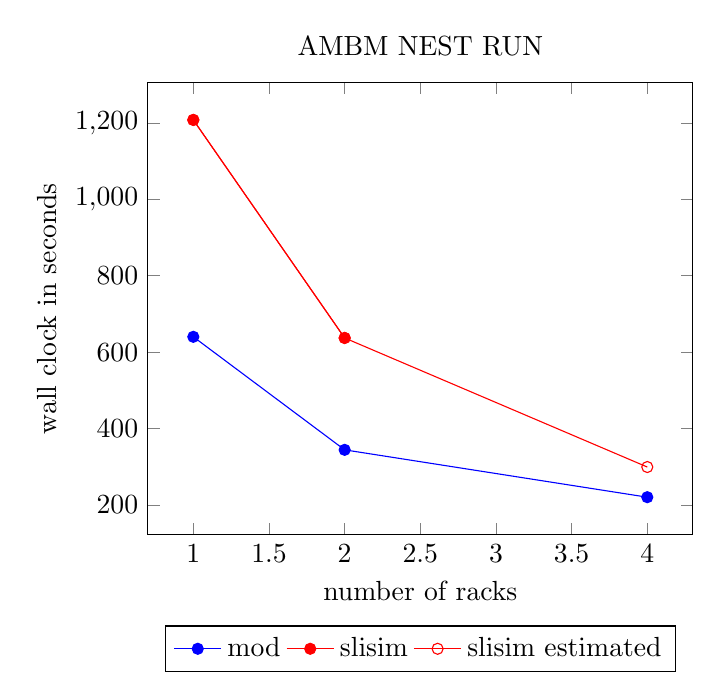
\begin{tikzpicture}
	\begin{axis}[title=AMBM NEST RUN,legend style={at={(0.5,-0.20)}, anchor=north,legend columns=-1},
		xlabel=number of racks,ylabel=wall clock in seconds,width=8.5cm]

	\addplot[color=blue,mark=*] coordinates {
		(1,640)
		(2,344)
		(4,220)
	};
	\addplot[color=red,mark=*] coordinates {
		(1,1208)
		(2,637)
	};
	\addplot[color=red,mark=o] coordinates {
		(1,1208)
		(2,637)
		(4,299)
	};
	\legend{mod,slisim, slisim estimated}
	\end{axis}%
\end{tikzpicture}%
\end{figure}

\begin{itemize}
      \item Tested in Lugano and Juelich
      \item Strong scaling
      \item Weak scaling
\end{itemize}

\subsection{Measured memory consumption}

\newpage
\subsection{Usability for Scientists}

\subsubsection{Manipulation of circuit}

\begin{itemize}
      \item control circuit generation / possibilities
      \item  manipulate circuit
\end{itemize}

\subsubsection{Import neurons}
\emph{H5NeuronCsX\_s\_s\_a\_s} expects 4 input parameters:
\begin{itemize}
      \item Name of the a subnet dataset (String).
The subset has to contain for each neuron an integer value.
The neurons are grouped together by this subnet value.

      \item A list of all datasets which values are interpreted as list of parameters.
      
      \item Name of the used neuron model
      
      \item path to the HDF5 file 
\end{itemize}
The function returns the neuron id of the first neuron it created.

\begin{lstlisting}[label=sliNeurons,caption=Calling the neuron import module via H5NeuronCsX\_s\_s\_a\_s SLI command ]
/neuronmodel /aeif_cond_exp def
/subnet (subnet) def
/neuronparams [(C_m) (Delta_T) (E_L) (V_reset) (V_th) (a) (b)] def
/filepath (circuit/ptneu_brain.h5) def
subnet neuronparams neuronmodel filepath H5NeuronCsX_s_s_a_s /offset Set
\end{lstlisting}



\begin{itemize}
      \item Sli command with parameters
      \item How can it be used
\end{itemize}

\subsubsection{Import synapses}
\emph{H5SynapseTll\_i\_s\_a\_s} expects 4 input parameters:
\begin{itemize}
      \item Offset of the neuron ids. Mostly it is equal to first neuron id returned by \emph{H5NeuronCsX\_s\_s\_a\_s}

      \item A list of all columns which values are interpreted as parameters.
      
      \item Name of the used synapse model
      
      \item path to the HDF5 file 
\end{itemize}
The function returns the neuron id of the first neuron it created.

\begin{lstlisting}[label=sliSynapses,caption=Example importing synapses]
/synmodel /tsodyks2_synapse def
/synparams [(delay) (weight) (U0) (TauRec) (TauFac)] def
/filepath (circuit/syn.h5) def
offset synparams synmodel filepath H5SynapseTll_i_s_a_s
\end{lstlisting}
\begin{itemize}
      \item Sli command with parameters
      \item How can it be used
\end{itemize}

\subsubsection{NEST simulation options}
\begin{itemize}
	  \item How to perform experiments
      \item Access neurons from imported circuit
      \item Test different stimuli 
\end{itemize}

\subsubsection{Analysis}
\begin{itemize}
	  \item Visualize spiking activity with Brion/Paraview
      \item Visualize spiking activity with ViSNEST
\end{itemize}




\end{document}
